%---------------------------------
%       REFERENCIAL TEÓRICO
%---------------------------------

\chapter[Referencial Teórico]{Referencial Teórico}


\section{Citação}

Citação 01 - ``Lorem Ipsum is simply dummy text of the printing and typesetting industry. Lorem Ipsum has been the'' \cite{AEB:20} \\\\
Citação 02 - Segundo \citeonline{Machado:11}, Lorem Ipsum is simply dummy text of the printing and typesetting industry.\\

\begin{citacao}
   Lorem Ipsum is simply dummy text of the printing and typesetting industry. Lorem Ipsum has been the industry's standard dummy text ever since the 1500s, when an unknown printer took a galley of type and scrambled it to make a type specimen book. It has survived. \cite{Sagan:19}
\end{citacao}

\begin{itemize}
    \item item 01;
    \item item 02;
    \item item 03.
\end{itemize}


\section{Figura}

\begin{figure}[ht]
    \caption{Contextualização da gamificação}
    \label{fig:game}
    \centering
    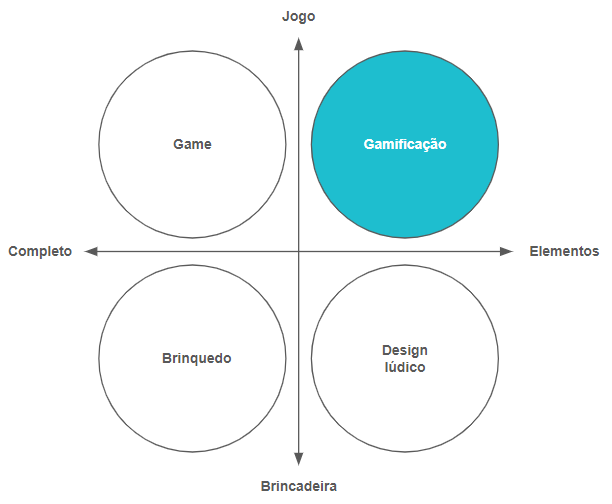
\includegraphics[width=0.5\textwidth]{figuras/Gamificação.png}
    \legend{Elaboração Própria}
\end{figure}


\section{Tabela}

\begin{table}[ht]
  \caption{Comparativo entre ferramentas similares}
  \label{Tab: Comparativo EA}
  \centering
  
  \begin{tabularx}{\textwidth}{p{4.4cm} ccccc}
    \hline
    \footnotesize\bfseries{Software} & \footnotesize\bfseries{Astronomia}   & \footnotesize\bfseries{Astronáutica}  & \footnotesize\bfseries{Mobile}  & \footnotesize\bfseries{Gamificação} & \footnotesize\bfseries{Português}\\
    \hline
    
        \footnotesize{Astronomia}              & x &   & x & x & x \\
        \footnotesize{Astronomy}               & x &   & x &   &   \\
        \footnotesize{Curso de Astronomia}     & x &   & x &   & x \\
        \footnotesize{ESApp}                   & x & x & x &   & x \\
        \footnotesize{Nasa}                    & x & x & x &   & x \\
        \footnotesize{Pockocmoc}               & x & x & x &   &   \\
        \footnotesize{Space Launch Now}        &   & x & x &   & x \\
        \footnotesize{Spacetoday}              & x & x &   &   & x \\
        \footnotesize{Stellarium}              & x &   & x &   & x \\
        \footnotesize{Space Learn}             & x & x & x & x & x \\ 
   
    \hline
  \end{tabularx}

  \legend{Elaboração Própria}
\end{table}




% https://www.seer.ufrgs.br/index.php/renote/article/view/53496/33013
% \footnotemark
% \footnotetext {Disponível em: <>. Acesso em: xx ______ xxxx.}
